% !TeX program = pdflatex
%==============================================================================
%  Aula 05 --- Métodos Não Paramétricos: Aspectos Teóricos
%  VERSÃO DO ALUNO: texto para leitura autônoma, fora da sala.
%  (O roteiro de sala é "05 Metodos Nao Parametricos Teoria.tex".)
%==============================================================================
\documentclass[11pt,a4paper]{article}
\usepackage[aluno]{../../recursos/latex/estilo-notas}

\title{}
\date{}

\begin{document}
\cabecalhoaula{05}{Métodos Não Paramétricos: Aspectos Teóricos}{AME §4.13 e cap.~5}

%==============================================================================
\section*{O que você vai aprender}
%==============================================================================
Ao final desta aula você deve ser capaz de:
\begin{itemize}[leftmargin=1.4cm]
  \item entender o que é uma \emph{taxa de convergência} e por que ela mede a
        qualidade de um estimador não paramétrico;
  \item enunciar as hipóteses de \emph{suavidade} (Lipschitz, Sobolev) e seu papel;
  \item deduzir a taxa de convergência do \textbf{KNN} via decomposição
        viés--variância;
  \item enunciar a taxa de \emph{séries ortogonais} e a noção de \emph{taxa
        minimax};
  \item explicar a \textbf{maldição da dimensionalidade} e sua consequência sobre o
        tamanho de amostra necessário;
  \item descrever as hipóteses de \emph{esparsidade} e \emph{redundância} e quais
        métodos se adaptam a elas.
\end{itemize}

\noindent
Esta aula responde \emph{por que} os métodos da Aula~04 funcionam --- e, mais
importante, \emph{quando não funcionam}. Kant tem uma frase que serve de lema:
\emph{``experiência sem teoria é cega''}. Guarde esta pergunta concreta, que ficará
sem resposta até a Seção~\ref{sec:esparsidade}:

\begin{center}\itshape
  no problema das resenhas da Amazon, por que o KNN foi tão pior\\
  que o Lasso e o \emph{boosting}?
\end{center}

\noindent
Não é detalhe de implementação nem azar de amostra. A resposta é inteiramente
teórica, e está nesta aula.

%==============================================================================
\section{Por que estudar taxas de convergência?}
%==============================================================================
Queremos comparar estimadores não pela performance em \emph{um} conjunto de dados,
mas pela rapidez com que o risco $\E[(\rhat(\X)-r(\X))^2]$ tende a zero conforme
$n\to\infty$. Uma \textbf{taxa de convergência} expressa esse decaimento em função
de $n$ (e da dimensão $p$, da suavidade etc.). Por exemplo, uma taxa $n^{-1/2}$ é
mais rápida (melhor) que $n^{-1/5}$.

\begin{ideia}
Estimação não paramétrica só é possível sob \textbf{suposições de suavidade}: se
$r$ pudesse oscilar arbitrariamente, nenhuma quantidade finita de dados a
determinaria. Suavidade é o que permite ``emprestar força'' de observações
vizinhas.
\end{ideia}

\noindent
Vale tornar isso concreto. Se $r$ pudesse valer qualquer coisa em cada ponto, saber
$r$ em mil pontos não diria \emph{nada} sobre $r$ num ponto novo --- e nenhum método
poderia funcionar. Toda a Aula~04 se apoia numa aposta implícita: pontos próximos em
$\x$ têm respostas próximas. Suavidade é essa aposta, escrita formalmente.

\noindent Duas medidas de suavidade que usaremos:
\begin{description}[leftmargin=2.2cm,style=nextline]
  \item[Lipschitz] $r$ é $L$-Lipschitz se
        $\abs{r(\x)-r(\x')}\le L\norm{\x-\x'}$ para todos $\x,\x'$. Controla
        \emph{quão rápido} $r$ pode variar. É a hipótese mínima: diz que andar uma
        distância $\delta$ não pode mudar $r$ em mais que $L\delta$.
  \item[Sobolev] $r$ tem suavidade $m$ se $\int (D^m r(x))^2\,dx \le K_1$
        ($m$ derivadas de quadrado integrável). Quanto maior $m$, mais suave.
\end{description}

%==============================================================================
\section{A taxa de convergência do KNN}
%==============================================================================
Considere o estimador KNN $\rhat_k(\x)=\frac1k\sum_{i\in\mathcal{N}_{\x}}Y_i$
(Aula~04). Sob suavidade Lipschitz, conseguimos limitar seu risco. O primeiro passo
é a peça central --- e a mais reveladora --- do argumento.

\begin{lema}[Distância média aos $k$ vizinhos]\label{lem:viz}
Se $\X$ é limitado e $p\ge 3$, então
\[
  \E\!\left[\Big(\frac1k\sum_{i\in\mathcal{N}_{\X}}\norm{\X_i-\X}\Big)^2\right]
  \le C\,\Big(\frac{k}{n}\Big)^{2/p}.
\]
\end{lema}

\begin{ideia}[de onde vem esse $2/p$]
O expoente não é mágica; é volume. Numa bola de raio $\rho$ em $\R^p$, o volume
cresce como $\rho^p$. Se os $n$ pontos estão espalhados num conjunto de volume $1$,
uma bola de raio $\rho$ contém, em média, $\approx n\rho^p$ deles. Para que ela
contenha os $k$ vizinhos que queremos, precisamos de $n\rho^p\approx k$, ou seja
\[
  \rho \;\approx\; \Big(\frac{k}{n}\Big)^{1/p}.
\]
Elevando ao quadrado (porque o lema fala do quadrado da distância) sai o
$(k/n)^{2/p}$. \textbf{Todo o resto da aula é consequência desse expoente $1/p$.}
\end{ideia}

\noindent
Em palavras: quanto mais vizinhos ($k$) eu exijo, mais \emph{longe} eles ficam. E o
$1/p$ no expoente diz que, em dimensão alta, essa distância cresce de forma
brutal --- a raiz $p$-ésima de um número pequeno está perto de $1$.

\begin{exemplo}[um número para sentir o problema]
Tome $n=10\,000$ pontos e $k=10$ vizinhos, num cubo de lado $1$. Então
$\rho\approx (10/10\,000)^{1/p} = (0{,}001)^{1/p}$:
\begin{center}\small
\renewcommand{\arraystretch}{1.2}
\begin{tabular}{@{}lccccc@{}}
\toprule
$p$ & $1$ & $2$ & $5$ & $10$ & $20$ \\
\midrule
raio $\rho$ necessário & $0{,}001$ & $0{,}032$ & $0{,}25$ & $0{,}50$ & $0{,}71$ \\
\bottomrule
\end{tabular}
\end{center}
Em $p=1$, os dez vizinhos cabem num intervalo de comprimento $0{,}001$: são
\emph{de fato} vizinhos. Em $p=20$, para reunir dez pontos você precisa de uma bola
que cobre \emph{setenta por cento} da largura do cubo --- ou seja, quase tudo. A
palavra ``vizinho'' perdeu o sentido, e com ela a justificativa do método.
\end{exemplo}

\begin{teorema}[Risco do KNN]\label{teo:knn}
Sob as hipóteses do Lema~\ref{lem:viz}, com $r$ $L$-Lipschitz e
$\sup_{\x}\Var(Y\mid\x)\le\sigma^2<\infty$,
\[
  \E\big[(\rhat_k(\X)-r(\X))^2\big]
   \;\le\; K\,\Big(\frac{k}{n}\Big)^{2/p} + \frac{\sigma^2}{k}.
\]
Otimizando em $k$ (tomando $k \asymp n^{2/(2+p)}$), obtém-se
\[
  \E\big[(\rhat_k(\X)-r(\X))^2\big] \;\le\; K'\, n^{-2/(2+p)}.
\]
\end{teorema}
\begin{proof}
Condicione nas covariáveis $\widetilde{\x}=(\x_1,\dots,\x_n,\x)$. Pela decomposição
viés--variância (Aula~01),
\[
  \E\big[(\rhat_k(\x)-r(\x))^2\mid\widetilde{\x}\big]
  = \underbrace{\Big(\tfrac1k\!\sum_{i\in\mathcal{N}_{\x}}\! r(\x_i)-r(\x)\Big)^2}_{\text{viés}^2}
  + \underbrace{\Var(\rhat_k(\x)\mid\widetilde{\x})}_{\text{variância}}.
\]
\emph{Viés:} como $r$ é $L$-Lipschitz,
$\big|\tfrac1k\sum_{i\in\mathcal{N}_{\x}}r(\x_i)-r(\x)\big|
\le \tfrac{L}{k}\sum_{i\in\mathcal{N}_{\x}}\norm{\x_i-\x}$.
\emph{Variância:} as respostas são independentes dadas as covariáveis e cada uma
tem variância $\le\sigma^2$; a média de $k$ delas tem variância
$\Var(\rhat_k(\x)\mid\widetilde{\x})\le \sigma^2/k$. Logo
\[
  \E\big[(\rhat_k(\x)-r(\x))^2\mid\widetilde{\x}\big]
  \le \Big(\tfrac{L}{k}\!\sum_{i\in\mathcal{N}_{\x}}\!\norm{\x_i-\x}\Big)^2 + \frac{\sigma^2}{k}.
\]
Tomando esperança e aplicando o Lema~\ref{lem:viz} ao primeiro termo, resulta
$\E[(\rhat_k(\X)-r(\X))^2]\le K(k/n)^{2/p}+\sigma^2/k$. Para minimizar em $k$,
iguale (a menos de constantes) os dois termos: $(k/n)^{2/p}\asymp 1/k$, isto é,
$k^{1+2/p}\asymp n^{2/p}$, ou seja $k\asymp n^{2/(2+p)}$, e substituindo obtém-se
a taxa $n^{-2/(2+p)}$.
\end{proof}

\begin{ideia}
A prova exibe explicitamente o balanço viés--variância da Aula~01: o termo
$(k/n)^{2/p}$ \emph{cresce} com $k$ (viés --- vizinhos mais distantes, respostas
menos parecidas com $r(\x)$) e $\sigma^2/k$ \emph{decresce} com $k$ (variância ---
média sobre mais observações). O $k$ ótimo equilibra os dois, e a validação cruzada
(Aula~03) é a maneira prática de encontrá-lo sem conhecer $L$, $\sigma^2$ nem $p$.
\end{ideia}

\begin{observacao}
O truque de ``igualar os dois termos'' para achar o $k$ ótimo merece uma nota: ele
funciona porque um termo cresce e o outro decresce em $k$, então o mínimo da soma
está onde eles se cruzam, a menos de constantes. É um recurso padrão em análise de
taxas, e você vai reencontrá-lo na próxima subseção com $J$ no lugar de $k$.
\end{observacao}

\subsection{Séries ortogonais e taxa minimax}
Para séries ortogonais (base de Fourier) com suavidade de Sobolev $m$, um argumento
análogo (viés do truncamento em $J$ termos $\le K_1 J^{-2m}$; variância $\le K_2 J/n$)
dá
\[
  \E\big[(\rhat_J(\X)-r(\X))^2\big] \le K_1 J^{-2m} + K_2\frac{J}{n},
  \quad\text{e com } J\asymp n^{1/(2m+1)}:\quad
  \E[\cdots] \le K\, n^{-2m/(2m+1)}.
\]
Note que mais suavidade ($m$ maior) $\Rightarrow$ taxa mais rápida.

\begin{observacao}[Taxa minimax]
Essas taxas não são apenas \emph{limitantes superiores} de um método específico:
para a classe $\mathcal{S}$ de funções suaves elas coincidem com a \textbf{taxa
minimax}
\[
  \inf_{\rhat}\ \sup_{r\in\mathcal{S}}\ \E\big[(\rhat(\X)-r(\X))^2\big]
  \asymp n^{-\alpha/(\alpha+p)},
\]
ou seja, \emph{nenhum} estimador faz essencialmente melhor no pior caso. Um
estimador que atinge essa taxa é dito \emph{minimax-ótimo}. ($\alpha$ liga-se à
suavidade.) Leia o $\inf_{\rhat}\sup_{r}$ como um jogo: você escolhe o estimador,
e um adversário, sabendo da sua escolha, escolhe a $r$ mais difícil dentro de
$\mathcal{S}$. A taxa minimax é o melhor que você garante contra o pior adversário.
Isso importa porque transforma a próxima seção de ``o KNN tem um problema'' em
``\emph{o problema} tem um problema''.
\end{observacao}

%==============================================================================
\section{A maldição da dimensionalidade}
%==============================================================================
Olhe a taxa minimax $n^{-\alpha/(\alpha+p)}$: para $p$ grande, o expoente
$\alpha/(\alpha+p)$ se aproxima de $0$ --- a convergência fica \emph{lentíssima}.

\begin{figure}[htbp]
  \centering
  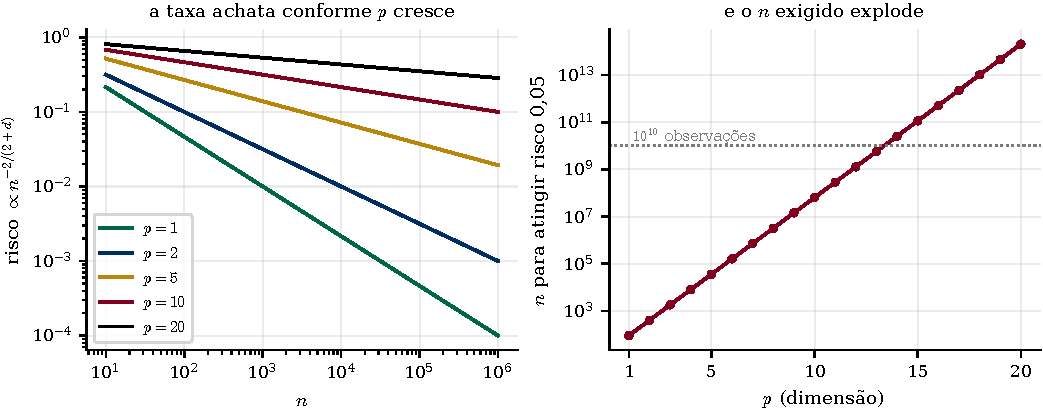
\includegraphics[width=\textwidth]{../../recursos/figuras/05-taxas.pdf}
  \caption{À esquerda, a taxa $n^{-2/(2+p)}$ em escala log--log: em $p=1$ a reta
  desce com inclinação $-2/3$; em $p=20$, com $-1/11$ --- quase horizontal. Aumentar
  a amostra deixa de adiantar. À direita, a leitura prática: quantas observações são
  necessárias para atingir risco $0{,}05$. Em $p=1$ bastam $90$; em $p=10$ já são
  $6{,}4\times10^{7}$; em $p=20$, $2\times10^{14}$ --- vinte e cinco mil vezes a
  população da Terra.}
  \label{fig:taxas}
\end{figure}

\begin{teorema}[Tamanho de amostra explode com $p$]
Para garantir risco $\le\delta$ na classe $\mathcal{S}$, é necessário
\[
  n \;\gtrsim\; \Big(\frac{K}{\delta}\Big)^{(\alpha+p)/\alpha},
\]
um crescimento \textbf{exponencial} em $p$.
\end{teorema}
Mesmo dimensões moderadas exigem amostras astronômicas. Esta é a
\textbf{maldição da dimensionalidade} (Bellman, 1966).

\begin{ideia}[A intuição da vizinhança vazia]
Para estimar $r(\x)$ por média local, preciso de pontos \emph{perto} de $\x$. Em
$\R^p$ com $p$ grande, qualquer vizinhança de raio fixo tem volume
desprezível: com alta probabilidade \emph{não há nenhum dado dentro dela}. Para
capturar $k$ vizinhos preciso de um raio $\asymp (k/n)^{1/p}$, que cresce com $p$
--- os ``vizinhos'' deixam de ser próximos, e o viés explode (é exatamente o
Lema~\ref{lem:viz}).
\end{ideia}

\noindent
Dá para medir isso diretamente, sem nenhuma teoria: espalhe $1000$ pontos ao acaso
num cubo $[0,1]^p$ e veja o quão longe fica o vizinho mais próximo de um ponto
qualquer (Figura~\ref{fig:vizinho}).

\begin{figure}[htbp]
  \centering
  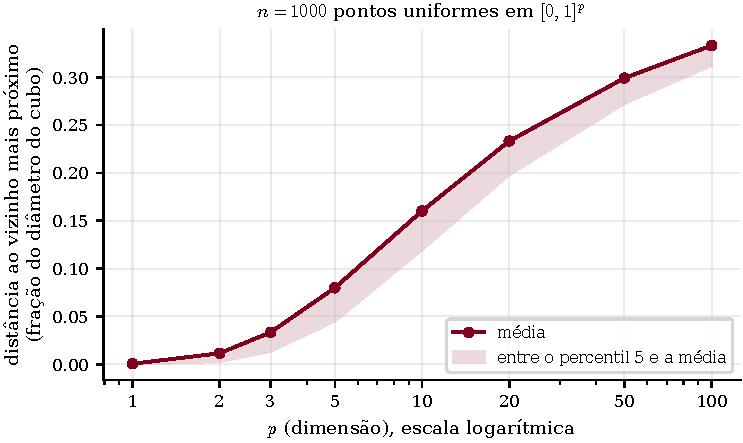
\includegraphics[width=0.72\textwidth]{../../recursos/figuras/05-vizinho-longe.pdf}
  \caption{Distância ao vizinho mais próximo entre $n=1000$ pontos uniformes em
  $[0,1]^p$, medida como fração do diâmetro do cubo. Em $p=1$ ela é praticamente
  zero; em $p=10$ já é $16\%$ do diâmetro; em $p=100$, um terço. Dito de outro modo:
  em dimensão alta \emph{todos os pontos estão a distâncias parecidas de todos os
  outros}, e ``os $k$ mais próximos'' vira uma seleção quase arbitrária.}
  \label{fig:vizinho}
\end{figure}

\begin{atencao}
A maldição diz que, \textbf{sem suposições extras}, estimação não paramétrica é
impossível em alta dimensão para $n$ realista. E, pela taxa minimax, a saída
\emph{não} é procurar um método melhor --- já sabemos que nenhum existe. A saída é
uma \emph{estrutura} adicional no problema, que tire a classe $\mathcal{S}$ do
pior caso. As duas mais úteis: esparsidade e redundância.
\end{atencao}

%==============================================================================
\section{Escapando da maldição}
%==============================================================================
\subsection{Esparsidade}\label{sec:esparsidade}
A hipótese de \textbf{esparsidade} diz que $r$ depende apenas de um subconjunto
$S\subset\{1,\dots,p\}$ de covariáveis:
\[
  r(\x) = r\big((x_i)_{i\in S}\big),\qquad \abs{S}=s \ll p.
\]
Embora haja $p$ covariáveis, só $s$ importam. Sob esparsidade a dimensão
\emph{efetiva} é $s$, e a taxa melhora para $\approx n^{-\alpha/(\alpha+s)}$.

Voltemos à pergunta da abertura. No problema das resenhas da Amazon, cada covariável
é a contagem de uma palavra, e a esmagadora maioria das palavras não diz nada sobre a
nota da resenha: o problema é \emph{esparso}. Isso explica os dois lados do
resultado:

\begin{itemize}[leftmargin=1.4cm]
  \item Métodos que \textbf{selecionam variáveis} --- Lasso (Aula~02), árvores e
        florestas, \emph{boosting} (Aula~06) --- descartam as irrelevantes e passam
        a operar na dimensão efetiva $s$. Para eles, o $p$ gigante quase não custa.
  \item O KNN \textbf{não faz seleção de variáveis}. Ele soma \emph{todas} as
        coordenadas na distância euclidiana, com peso igual. Cada palavra
        irrelevante acrescenta ruído à distância, e com milhares delas a distância
        passa a medir essencialmente ruído. Os ``vizinhos'' encontrados não são
        vizinhos no que importa.
\end{itemize}

\begin{ideia}
Este é o ponto da aula que mais vale levar: o KNN não perdeu por ser fraco, e sim
por ser \emph{indiferente à estrutura do problema}. Um método que trata todas as
covariáveis igualmente está apostando que todas importam igualmente --- e quando
essa aposta está errada, ele paga o preço integral da dimensão $p$, mesmo que a
dimensão efetiva seja $s=20$.
\end{ideia}

\begin{observacao}
Métodos que se adaptam à esparsidade: \emph{Lasso} (Aula~02), \emph{florestas
aleatórias} (cuja taxa, por Biau 2012, depende só do número de variáveis
relevantes, pois divisões inúteis raramente são escolhidas) e \emph{SpAM}
(modelos aditivos esparsos, que combinam aditividade com $\ell_1$).
\end{observacao}

\subsection{Redundância}
A hipótese de \textbf{redundância} diz que as covariáveis, embora em número $p$,
vivem (aproximadamente) sobre uma \emph{subvariedade} de dimensão intrínseca
$u\ll p$. Exemplos:
\begin{itemize}[leftmargin=1.4cm,nosep]
  \item altura, peso e IMC: três variáveis, mas duas determinam a terceira;
  \item imagens: \emph{pixels} adjacentes são quase iguais --- enorme redundância.
\end{itemize}
Sob redundância, KNN e regressão local \emph{se adaptam automaticamente} à dimensão
intrínseca: sua taxa passa a ser $n^{-4/(4+u)}$, muito mais rápida que
$n^{-4/(4+p)}$ quando $u\ll p$. SVR com kernel gaussiano e séries \emph{espectrais}
(base construída a partir dos dados) também exploram redundância.

\begin{ideia}
Esparsidade $\neq$ redundância, e a diferença decide o método.
\emph{Esparsidade}: poucas covariáveis importam, as demais são lixo --- seleção de
variáveis ajuda, e o KNN não se salva. \emph{Redundância}: todas podem importar,
mas elas são correlacionadas e os dados ocupam só uma fatia fina do espaço --- aqui
o KNN \emph{se vira bem sozinho}, porque os vizinhos são medidos dentro da
subvariedade, e a redução de dimensionalidade (PCA, aula extra) ajuda ainda mais.
\end{ideia}

%==============================================================================
\section{Síntese prática}
%==============================================================================
\begin{center}\small
\renewcommand{\arraystretch}{1.3}
\begin{tabular}{@{}lll@{}}
\toprule
\textbf{Situação} & \textbf{O que ajuda} & \textbf{Métodos} \\
\midrule
$p$ pequeno, $r$ suave & nada extra & KNN, NW, regressão local \\
Poucas covariáveis relevantes & seleção de variáveis & Lasso, florestas, XGBoost, SpAM \\
Covariáveis redundantes & dimensão intrínseca & KNN/local, SVR, séries espectrais, PCA \\
\bottomrule
\end{tabular}
\end{center}

O notebook \texttt{Aula prática 05} é um laboratório de simulação: mede o expoente
$1/p$ do raio que reúne $k$ vizinhos, estima a taxa de convergência do KNN em
$p=1,2,4,8$, abre o risco em viés$^2$ e variância para ver as duas parcelas se
cruzarem no $k$ ótimo, e separa esparsidade de redundância medindo a dimensão
intrínseca --- inclusive a do \texttt{superconductivity.csv}.

\begin{atencao}
Mensagem para levar para casa: \textbf{não existe almoço grátis}. A escolha do
método deve refletir a \emph{estrutura} que você acredita existir nos dados. A
teoria desta aula é o que torna essa escolha informada em vez de adivinhação --- e
é também o que impede você de culpar a implementação quando um método vai mal por
razões que eram previsíveis no papel.
\end{atencao}

%==============================================================================
\section*{Resumo}
%==============================================================================
\begin{itemize}[leftmargin=1.4cm]
  \item Taxas de convergência medem a qualidade assintótica; só existem sob
        \emph{suavidade} (Lipschitz, Sobolev).
  \item KNN: risco $\le K(k/n)^{2/p}+\sigma^2/k$, ótimo em
        $k\asymp n^{2/(2+p)}$, taxa $n^{-2/(2+p)}$ (Teo.~\ref{teo:knn}). O expoente
        $1/p$ nasce do volume da bola em $\R^p$ (Lema~\ref{lem:viz}).
  \item Séries ($m$-suaves): taxa $n^{-2m/(2m+1)}$; ambas atingem a taxa
        \emph{minimax} $n^{-\alpha/(\alpha+p)}$ --- ou seja, não há método melhor.
  \item \textbf{Maldição da dimensionalidade}: a taxa degrada com $p$
        (Fig.~\ref{fig:taxas}) e os vizinhos deixam de ser vizinhos
        (Fig.~\ref{fig:vizinho}).
  \item \emph{Esparsidade} (poucas relevantes) $\to$ Lasso/florestas; o KNN vai mal
        porque usa todas as covariáveis com peso igual. \emph{Redundância}
        (dimensão intrínseca baixa) $\to$ KNN/local, séries espectrais, PCA.
\end{itemize}

\paragraph{Leitura recomendada.} [AME] §4.13 (as contas de taxa do KNN e das séries
ortogonais, das quais o Teo.~\ref{teo:knn} desta aula é a versão detalhada) e
Capítulo~5 inteiro: §5.1 (maldição da dimensionalidade e taxas), §5.1.1
(esparsidade), §5.1.2 (redundância), §5.2 (KNN e regressão local sob redundância) e
§5.5--5.6 (florestas aleatórias e SpAM).

\paragraph{Para praticar.} \texttt{Lista teorica 05.pdf} (teórica, com gabarito) e \texttt{Lista prática 05.ipynb} (prática, para completar as lacunas), nesta mesma pasta.

\end{document}
